\documentclass[letterpaper,12pt]{article}\usepackage[]{graphicx}\usepackage[]{color}
%% maxwidth is the original width if it is less than linewidth
%% otherwise use linewidth (to make sure the graphics do not exceed the margin)
\makeatletter
\def\maxwidth{ %
  \ifdim\Gin@nat@width>\linewidth
    \linewidth
  \else
    \Gin@nat@width
  \fi
}
\makeatother

\definecolor{fgcolor}{rgb}{0.345, 0.345, 0.345}
\newcommand{\hlnum}[1]{\textcolor[rgb]{0.686,0.059,0.569}{#1}}%
\newcommand{\hlstr}[1]{\textcolor[rgb]{0.192,0.494,0.8}{#1}}%
\newcommand{\hlcom}[1]{\textcolor[rgb]{0.678,0.584,0.686}{\textit{#1}}}%
\newcommand{\hlopt}[1]{\textcolor[rgb]{0,0,0}{#1}}%
\newcommand{\hlstd}[1]{\textcolor[rgb]{0.345,0.345,0.345}{#1}}%
\newcommand{\hlkwa}[1]{\textcolor[rgb]{0.161,0.373,0.58}{\textbf{#1}}}%
\newcommand{\hlkwb}[1]{\textcolor[rgb]{0.69,0.353,0.396}{#1}}%
\newcommand{\hlkwc}[1]{\textcolor[rgb]{0.333,0.667,0.333}{#1}}%
\newcommand{\hlkwd}[1]{\textcolor[rgb]{0.737,0.353,0.396}{\textbf{#1}}}%

\usepackage{framed}
\makeatletter
\newenvironment{kframe}{%
 \def\at@end@of@kframe{}%
 \ifinner\ifhmode%
  \def\at@end@of@kframe{\end{minipage}}%
  \begin{minipage}{\columnwidth}%
 \fi\fi%
 \def\FrameCommand##1{\hskip\@totalleftmargin \hskip-\fboxsep
 \colorbox{shadecolor}{##1}\hskip-\fboxsep
     % There is no \\@totalrightmargin, so:
     \hskip-\linewidth \hskip-\@totalleftmargin \hskip\columnwidth}%
 \MakeFramed {\advance\hsize-\width
   \@totalleftmargin\z@ \linewidth\hsize
   \@setminipage}}%
 {\par\unskip\endMakeFramed%
 \at@end@of@kframe}
\makeatother

\definecolor{shadecolor}{rgb}{.97, .97, .97}
\definecolor{messagecolor}{rgb}{0, 0, 0}
\definecolor{warningcolor}{rgb}{1, 0, 1}
\definecolor{errorcolor}{rgb}{1, 0, 0}
\newenvironment{knitrout}{}{} % an empty environment to be redefined in TeX

\usepackage{alltt}
\usepackage[top=1in,bottom=1in,left=1in,right=1in]{geometry}
\usepackage{setspace}
\usepackage[colorlinks=true,urlcolor=blue,citecolor=blue,linkcolor=blue]{hyperref}
\usepackage{indentfirst}
\usepackage{multirow}
\usepackage{booktabs}
\usepackage[final]{animate}
\usepackage{graphicx}
\usepackage{verbatim}
\usepackage{rotating}
\usepackage{tabularx}
\usepackage{array}
\usepackage{subfig} 
\usepackage[noae]{Sweave}
\usepackage{cleveref}
\usepackage[figureposition=bottom]{caption}
\usepackage{paralist}
\usepackage{acronym}
\usepackage{outlines}
\usepackage{pdflscape}

% knitr options


\IfFileExists{upquote.sty}{\usepackage{upquote}}{}
\begin{document}

\setlength{\parskip}{5mm}
\setlength{\parindent}{0in}

\title{Summary of data processing for Patuxent River Estuary}
\author{Marcus W. Beck, Rebecca Murphy}
\maketitle

The following describes additional processing of raw station data for the Patuxent River Estuary. Briefs descriptions of each step are provided.

The following raw data files were imported:
\begin{enumerate}
\item \texttt{PAX\_TRIB\_CHLAandSALINITY\_85to14.csv}: chlorophyll and salinity data for all stations in the Patuxent River from 1985 to 2014 (from R. Murphy)
\item \texttt{PAX\_station\_info.csv}: metadata for each station including lat/lon, salinity zone, etc. (from R. Murphy)
\item \texttt{cb5\_1\_w.csv}: Salinity data for all depth zones at station CB5.1W at the outflow of the Patuxent River Estuary, used to calculate fraction of freshwater
\end{enumerate}

The data were first imported into R.
\begin{kframe}
\begin{alltt}
\hlcom{# code for processing raw data, see email from R. Murphy on 3/13/15}
\hlcom{# created March 2015, M. Beck}

\hlcom{## packages to use}
\hlcom{# this is just to load dplyr, ggplot2}
\hlstd{devtools}\hlopt{::}\hlkwd{load_all}\hlstd{(}\hlstr{'M:/docs/tidal_comp/TidalComp'}\hlstd{)}

\hlcom{## import}

\hlcom{# meta}
\hlstd{pax_meta} \hlkwb{<-} \hlkwd{system.file}\hlstd{(}\hlstr{'PAX_station_info.csv'}\hlstd{,} \hlkwc{package} \hlstd{=} \hlstr{'TidalComp'}\hlstd{)}
\hlstd{pax_meta} \hlkwb{<-} \hlkwd{read.csv}\hlstd{(pax_meta,} \hlkwc{header} \hlstd{=} \hlnum{TRUE}\hlstd{,}
  \hlkwc{stringsAsFactors} \hlstd{=} \hlnum{FALSE}\hlstd{)}

\hlcom{# data}
\hlstd{pax_data} \hlkwb{<-} \hlkwd{system.file}\hlstd{(}\hlstr{'PAX_TRIB_CHLAandSALINITY_85to14.csv'}\hlstd{,}
  \hlkwc{package} \hlstd{=} \hlstr{'TidalComp'}\hlstd{)}
\hlstd{pax_data} \hlkwb{<-} \hlkwd{read.csv}\hlstd{(pax_data,} \hlkwc{header} \hlstd{=} \hlnum{TRUE}\hlstd{,}
  \hlkwc{stringsAsFactors} \hlstd{=} \hlnum{FALSE}\hlstd{)}

\hlcom{# reorder STATION variable along trib axis}
\hlstd{stats} \hlkwb{<-} \hlkwd{c}\hlstd{(}\hlstr{'TF1.0'}\hlstd{,} \hlstr{'TF1.3'}\hlstd{,} \hlstr{'TF1.4'}\hlstd{,} \hlstr{'TF1.5'}\hlstd{,} \hlstr{'TF1.6'}\hlstd{,} \hlstr{'TF1.7'}\hlstd{,}
  \hlstr{'RET1.1'}\hlstd{,} \hlstr{'LE1.1'}\hlstd{,} \hlstr{'LE1.2'}\hlstd{,} \hlstr{'LE1.3'}\hlstd{,} \hlstr{'LE1.4'}\hlstd{)}
\hlstd{pax_data}\hlopt{$}\hlstd{STATION} \hlkwb{<-} \hlkwd{factor}\hlstd{(pax_data}\hlopt{$}\hlstd{STATION,} \hlkwc{level} \hlstd{= stats)}

\hlcom{# most seaward station for fraction of freshwater}
\hlstd{ffw_data} \hlkwb{<-} \hlkwd{system.file}\hlstd{(}\hlstr{'cb5_1_w.csv'}\hlstd{,} \hlkwc{package} \hlstd{=} \hlstr{'TidalComp'}\hlstd{)}
\hlstd{ffw_data} \hlkwb{<-} \hlkwd{read.csv}\hlstd{(ffw_data,} \hlkwc{header} \hlstd{=} \hlnum{TRUE}\hlstd{,}
  \hlkwc{stringsAsFactors} \hlstd{=} \hlnum{FALSE}\hlstd{)}
\end{alltt}
\end{kframe}

Salinity data (ppt) at the most seaward station (CB5.1W) were vertically integrated for each unique date.  The integration function averaged all salinity values after interpolating from the surface to the maximum depth.  Salinity values at the most shallow and deepest sampling depth were repeated for zero depth and maximum depths, respectively, to bound the interpolations within the range of the data.  A moving window average was also used to aggregate salinity values for all preceding two months for each observation.  This approach was used to account for lags in water exchange near the estuary mouth with the mainstem based on previously estimated residence times.  
\begin{kframe}
\begin{alltt}
\hlcom{##}
\hlcom{# process CB5.1W data for fraction of freshwater}

\hlcom{# vertical integration by date, station}
\hlstd{int_fun} \hlkwb{<-} \hlkwa{function}\hlstd{(}\hlkwc{TOTAL_DEPTH}\hlstd{,} \hlkwc{DEPTH}\hlstd{,} \hlkwc{VALUE}\hlstd{)\{}

  \hlkwa{if}\hlstd{(}\hlkwd{length}\hlstd{(}\hlkwd{na.omit}\hlstd{(VALUE))} \hlopt{<} \hlnum{2} \hlstd{)} \hlkwd{return}\hlstd{(}\hlkwd{na.omit}\hlstd{(VALUE))}

  \hlcom{# setup for interpolation}
  \hlstd{max_depths} \hlkwb{<-} \hlkwd{mean}\hlstd{(}\hlkwd{unique}\hlstd{(TOTAL_DEPTH),} \hlkwc{na.rm} \hlstd{=} \hlnum{TRUE}\hlstd{)}
  \hlstd{depths} \hlkwb{<-} \hlkwd{c}\hlstd{(}\hlnum{0}\hlstd{, DEPTH, max_depths)}
  \hlstd{vals} \hlkwb{<-} \hlkwd{c}\hlstd{(VALUE[}\hlnum{1}\hlstd{], VALUE, VALUE[}\hlkwd{length}\hlstd{(VALUE)])}

  \hlcom{# only interpolate if > 1 salinity value}
  \hlstd{out} \hlkwb{<-} \hlkwd{mean}\hlstd{(}\hlkwd{approx}\hlstd{(depths, vals)}\hlopt{$}\hlstd{y)}

  \hlkwd{return}\hlstd{(out)}

  \hlstd{\}}

\hlcom{# for filter}
\hlstd{wins} \hlkwb{<-} \hlnum{2}\hlcom{# 2 months}
\hlstd{wins} \hlkwb{<-} \hlkwd{rep}\hlstd{(}\hlnum{1}\hlstd{,} \hlkwc{length} \hlstd{= wins)}\hlopt{/}\hlstd{wins}

\hlcom{# process}
\hlstd{ffw_data} \hlkwb{<-} \hlkwd{select}\hlstd{(ffw_data, SAMPLE_DATE, DEPTH, VALUE, TOTAL_DEPTH)} \hlopt
  \hlkwd{group_by}\hlstd{(SAMPLE_DATE)} \hlopt
  \hlkwd{summarize}\hlstd{(}\hlkwc{sal_ref} \hlstd{=} \hlkwd{int_fun}\hlstd{(TOTAL_DEPTH, DEPTH, VALUE))} \hlopt
  \hlstd{na.omit} \hlopt
  \hlkwd{mutate}\hlstd{(}\hlkwc{date} \hlstd{=} \hlkwd{as.Date}\hlstd{(SAMPLE_DATE,} \hlstr{'%m/%d/%Y'}\hlstd{))} \hlopt
  \hlkwd{select}\hlstd{(date, sal_ref)} \hlopt
  \hlkwd{arrange}\hlstd{(date)} \hlopt
  \hlkwd{mutate}\hlstd{(}\hlkwc{sal_ref} \hlstd{= stats}\hlopt{::}\hlkwd{filter}\hlstd{(sal_ref, wins,} \hlkwc{sides} \hlstd{=} \hlnum{1}\hlstd{))}
\end{alltt}
\end{kframe}

A similar process for vertically-integrating salinity across depth values was used for the remaining station data.
\begin{kframe}
\begin{alltt}
\hlcom{##}
\hlcom{# get vertically integrated salinity as before}

\hlcom{# process}
\hlcom{# note that there are no 'PROBLEM' values, lab and method do not change}
\hlstd{sal_tmp} \hlkwb{<-} \hlkwd{filter}\hlstd{(pax_data, PARAMETER} \hlopt{==} \hlstr{'SALINITY'}\hlstd{)} \hlopt
  \hlkwd{mutate}\hlstd{(}\hlkwc{date} \hlstd{=} \hlkwd{as.Date}\hlstd{(date,} \hlkwc{format} \hlstd{=} \hlstr{'%m/%d/%Y'}\hlstd{))} \hlopt
  \hlkwd{group_by}\hlstd{(date, STATION)} \hlopt
  \hlkwd{summarize}\hlstd{(}\hlkwc{sal} \hlstd{=} \hlkwd{int_fun}\hlstd{(TOTAL_DEPTH, DEPTH, AvgValue))}
\end{alltt}
\end{kframe}

Chlorophyll values at each station were retained only for surface samples and no `problem' codes.  Chlorophyll were also transformed by the natural-log.  
\begin{kframe}
\begin{alltt}
\hlcom{##}
\hlcom{# get only surface estimates for chlorophyll}
\hlcom{# remove those w/ problem codes}
\hlstd{chl_tmp} \hlkwb{<-} \hlkwd{filter}\hlstd{(pax_data,}
  \hlstd{PARAMETER} \hlopt{==} \hlstr{'CHLA'} \hlopt{&} \hlstd{LAYER} \hlopt{==} \hlstr{'S'}\hlopt{&} \hlstd{PROBLEM} \hlopt{==} \hlstr{''}
  \hlstd{)} \hlopt
  \hlkwd{mutate}\hlstd{(}\hlkwc{lnchla} \hlstd{=} \hlkwd{log}\hlstd{(AvgValue))} \hlopt
  \hlkwd{mutate}\hlstd{(}\hlkwc{date} \hlstd{=} \hlkwd{as.Date}\hlstd{(date,} \hlkwc{format} \hlstd{=} \hlstr{'%m/%d/%Y'}\hlstd{))} \hlopt
  \hlkwd{select}\hlstd{(date, STATION, lnchla)}
\end{alltt}
\end{kframe}

The reference salinity data at CB5.1W was merged with the salinity data at each date and station to estimate fraction of freshwater.  Sample dates between the reference station and all remaining stations were similar, although in some cases the dates did not match exactly.  Again, linear interpolation was used to fill in missing observation dates for salinity at the reference site to match with observation dates at the remaining stations.  The corresponding plot shows dates at each station that required interpolation at the reference station. 
\begin{kframe}
\begin{alltt}
\hlcom{##}
\hlcom{# ref salinity dates for CB5.1W need to match sample dates from rest of trib}
\hlcom{# CB5.1W data are merged with all vertically-integrated salinity data}
\hlcom{# missing dates for CB5.1W are interpolated to get matches}

\hlstd{int_fun} \hlkwb{<-}  \hlkwa{function}\hlstd{(}\hlkwc{date}\hlstd{,} \hlkwc{sal_ref}\hlstd{)\{}
  \hlstd{interps} \hlkwb{<-} \hlkwd{approx}\hlstd{(}\hlkwc{x} \hlstd{= date,} \hlkwc{y}  \hlstd{= sal_ref,} \hlkwc{xout} \hlstd{= date)}\hlopt{$}\hlstd{y}
  \hlstd{sal_ref[}\hlkwd{is.na}\hlstd{(sal_ref)]} \hlkwb{<-} \hlstd{interps[}\hlkwd{is.na}\hlstd{(sal_ref)]}
  \hlkwd{return}\hlstd{(sal_ref)}
\hlstd{\}}

\hlstd{sal_mrg} \hlkwb{<-} \hlkwd{full_join}\hlstd{(sal_tmp, ffw_data,} \hlkwc{by} \hlstd{=} \hlstr{'date'}\hlstd{)} \hlopt \hlcom{# merge}
  \hlstd{ungroup} \hlopt
  \hlkwd{arrange}\hlstd{(STATION, date)} \hlopt \hlcom{# sort by station, date}
  \hlkwd{group_by}\hlstd{(STATION)} \hlopt
  \hlkwd{mutate}\hlstd{(}\hlkwc{sal_ref_int} \hlstd{=} \hlkwd{int_fun}\hlstd{(date, sal_ref))}

\hlcom{# plot the interpolated values to see if they're ok}
\hlcom{# red lines are values that were interpolated}
\hlkwd{ggplot}\hlstd{(sal_mrg,} \hlkwd{aes}\hlstd{(}\hlkwc{x} \hlstd{= date,} \hlkwc{y} \hlstd{= sal_ref_int,} \hlkwc{group} \hlstd{= STATION))} \hlopt{+}
  \hlkwd{geom_line}\hlstd{(}\hlkwc{colour} \hlstd{=} \hlstr{'red'}\hlstd{,} \hlkwc{size} \hlstd{=} \hlnum{0.3}\hlstd{)} \hlopt{+}
  \hlkwd{geom_line}\hlstd{(}\hlkwd{aes}\hlstd{(}\hlkwc{y} \hlstd{= sal_ref))} \hlopt{+}
  \hlkwd{facet_wrap}\hlstd{(}\hlopt{~}\hlstd{STATION,} \hlkwc{ncol} \hlstd{=} \hlnum{3}\hlstd{)} \hlopt{+}
  \hlkwd{theme_classic}\hlstd{()}
\end{alltt}
\end{kframe}

{\centering 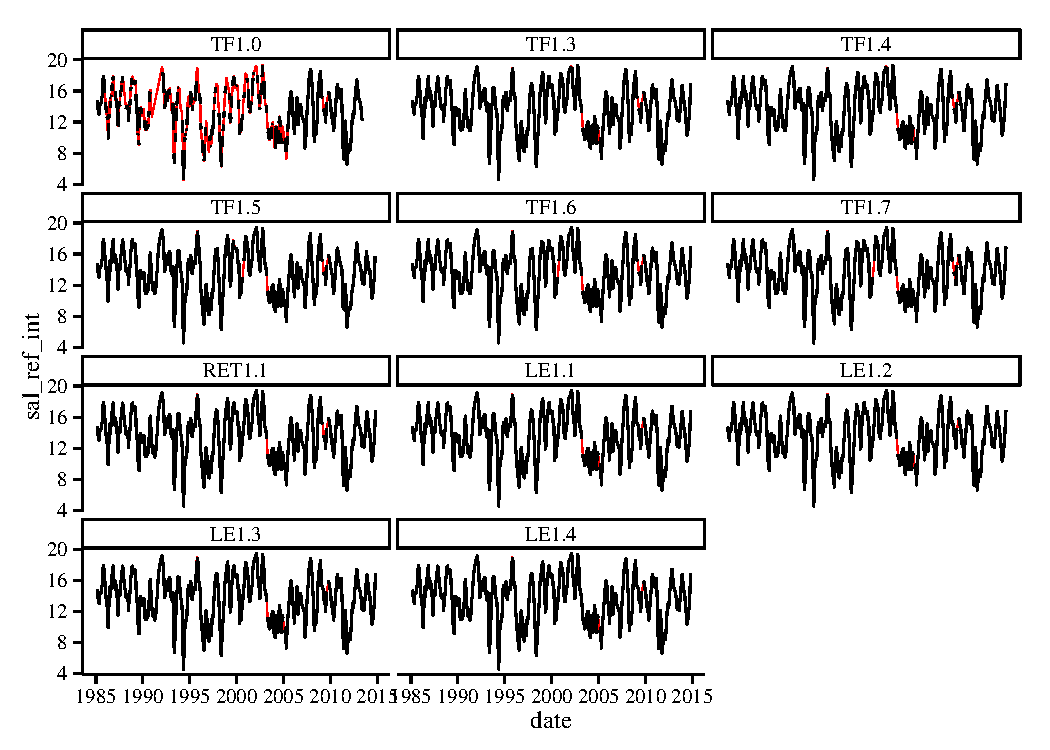
\includegraphics[width=\maxwidth]{figs/unnamed-chunk-5} 

}




The fraction of freshwater data were merged with the chlorophyll data.  All unique data were retained.
\begin{kframe}
\begin{alltt}
\hlcom{## }
\hlcom{# merge chl and salinity data}
\hlcom{# create fraction of freshwater}

\hlstd{pax_data} \hlkwb{<-} \hlkwd{full_join}\hlstd{(chl_tmp, sal_mrg,} \hlkwc{by} \hlstd{=} \hlkwd{c}\hlstd{(}\hlstr{'date'}\hlstd{,} \hlstr{'STATION'}\hlstd{))} \hlopt
  \hlkwd{mutate}\hlstd{(}\hlkwc{salff} \hlstd{=} \hlnum{1} \hlopt{-} \hlstd{sal}\hlopt{/}\hlstd{sal_ref_int)}

\hlkwd{ggplot}\hlstd{(pax_data,} \hlkwd{aes}\hlstd{(}\hlkwc{x} \hlstd{= date,} \hlkwc{y} \hlstd{= salff,} \hlkwc{group} \hlstd{= STATION))} \hlopt{+}
  \hlkwd{geom_line}\hlstd{()} \hlopt{+}
  \hlkwd{theme_classic}\hlstd{()} \hlopt{+}
  \hlkwd{geom_hline}\hlstd{(}\hlkwc{yintercept} \hlstd{=} \hlnum{0}\hlstd{,} \hlkwc{colour} \hlstd{=} \hlstr{'blue'}\hlstd{,} \hlkwc{linetype} \hlstd{=} \hlstr{'dashed'}\hlstd{)} \hlopt{+}
  \hlkwd{facet_wrap}\hlstd{(}\hlopt{~} \hlstd{STATION,} \hlkwc{ncol} \hlstd{=} \hlnum{3}\hlstd{)}

\hlkwd{ggplot}\hlstd{(pax_data,} \hlkwd{aes}\hlstd{(}\hlkwc{x} \hlstd{= date,} \hlkwc{y} \hlstd{= lnchla,} \hlkwc{group} \hlstd{= STATION))} \hlopt{+}
  \hlkwd{geom_line}\hlstd{()} \hlopt{+}
  \hlkwd{theme_classic}\hlstd{()} \hlopt{+}
  \hlkwd{facet_wrap}\hlstd{(}\hlopt{~} \hlstd{STATION,} \hlkwc{ncol} \hlstd{=} \hlnum{3}\hlstd{)}
\end{alltt}
\end{kframe}

{\centering 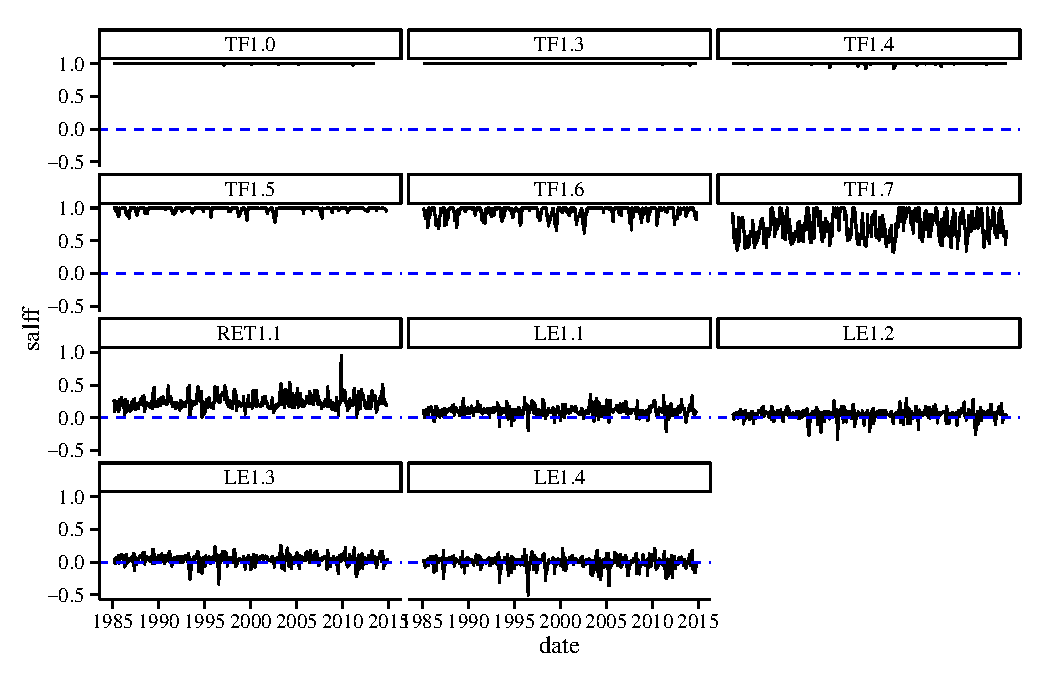
\includegraphics[width=\maxwidth]{figs/unnamed-chunk-61} 
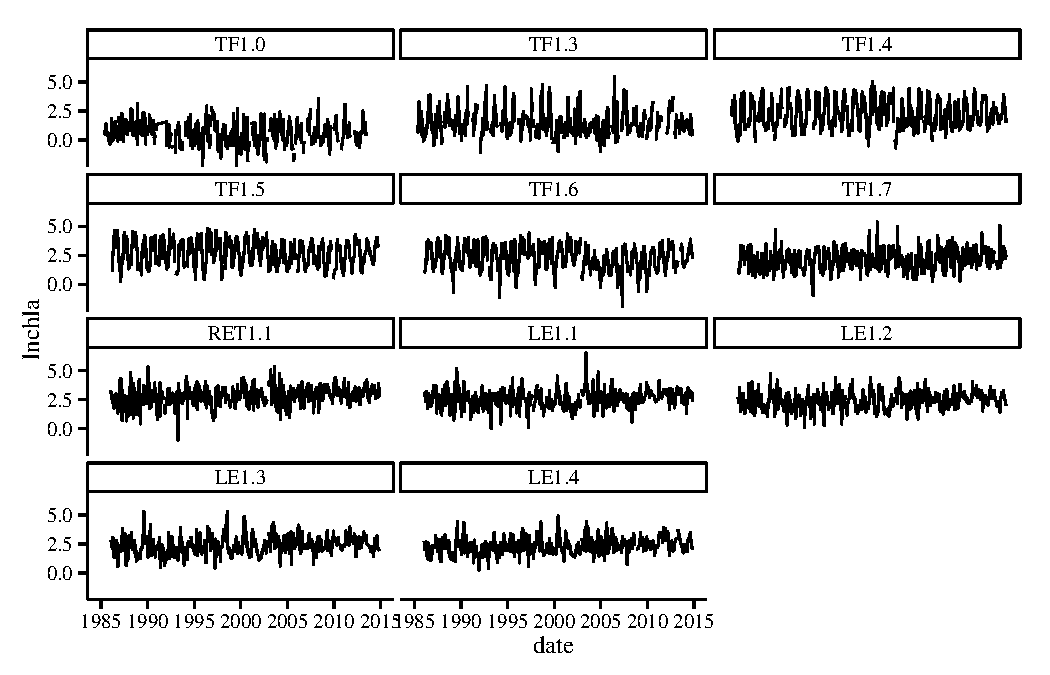
\includegraphics[width=\maxwidth]{figs/unnamed-chunk-62} 

}




\end{document}
